%!TEX = xelatex
\documentclass[conference]{IEEEtran}
\IEEEoverridecommandlockouts
\usepackage[style=ieee]{biblatex}
    \addbibresource{references.bib
}
\usepackage{graphicx}
\usepackage{amsmath}
\usepackage{amssymb}
\usepackage{xcolor}
    \newcommand{\todo}[1]{\textcolor{red}{[ #1 ]}}
    \newcommand{\instruction}[1]{\textcolor{orange}{#1}}
% \renewcommand{\todo}[1]{} % Uncomment to hide todos.
% \renewcommand{\instruction}[1]{} % Uncomment to hide instructions.

\newcommand{\hidden}[1]{}

\usepackage[colorlinks=false]{hyperref}

\title{STATS 402 - Interdisciplinary Data Analysis\\
    Resource-Constrained Deep Reinforcement Learning for Battlesnake
}
\author{\IEEEauthorblockN{Steven Hé (Sīchàng)\\
    sichang.he@dukekunshan.edu.cn
}}

\begin{document}
\maketitle

\begin{abstract}
    \instruction{Insert a very brief paragraph describing your project (300 words)}

    \todo{the actual problem you are considering and the motivation behind your method;}

    \todo{brief description of the method you designed;}

    \todo{brief description of how you validated the method you proposed.}
\end{abstract}

\section{Introduction}

\todo{briefly introduce the background knowledge of the actual problem
    you want to solve and the motivation behind your design
}

\todo{briefly introduce the characteristics of your method}

Battlesnake~\cite{battlesnake}
is a popular online programming competition in the form of a simultaneous
multiplayer board game. Similar to the arcade snake game,
each player controls a snake in real time on a finite grid board to be the last
one alive; the snake can change directions within each turn,
grow in length by eating randomly spawned food,
die from colliding with walls or snake bodies,
or starve to death after not eating for a long time (100 turns),
as demonstrated in Fig.~\ref{fig:game}.
Instead of having human players control the snakes, in Battlesnake,
players develop a computer program to control their snakes' directions in each
turn, by implementing a web server that responds to the game server's request,
which contains the entire game state.
This means players can implement their algorithms freely,
as long as they can finish the response within the time limitation (500ms).

\begin{figure}
    \centering
    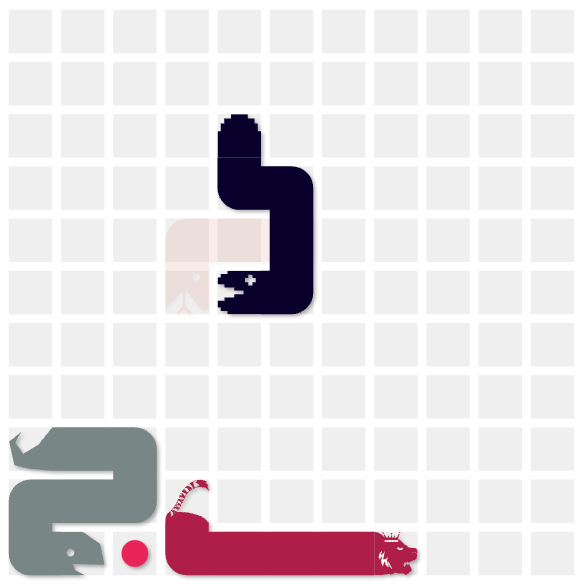
\includegraphics[width=\linewidth]{snake_game_screenshot.png}
    \caption{A Standard Battlesnake Game with 4 Snakes on A 11x11 Board.
        The transparent snake is already dead.
    }
    \label{fig:game}
\end{figure}

Battlesnake is an ideal target for implementing deep reinforcement learning.
Traditionally,
the leader board is occupied by players employing various heuristics and Monte
Carlo tree search algorithms,
most notably minimax~\cite{hill2018building,binnersley2020battlesnake}. However,
more recently,
even well-defined heuristics and tree search algorithms are only adequate for
intermediate-level gameplay~\cite{schier2019adversarial}. Additionally,
given the large search space (over $(3^n)^t$ raw possibilities for $t$ turns in
a game with $n$ snakes),
tree search algorithms are computationally demanding even when techniques like
alpha-beta pruning are employed. This cost problem is magnified,
especially considering the game sets a 500ms action time limit.
To address these problems, we compare Battlesnake to the game of Go,
which also has a large possibility space and potentially long time horizon,
and AlphaGo has demonstrated that deep reinforcement learning can excel in such
situations and achieve superhuman-level performance~\cite{silver2016mastering}.
More recent examples of deep reinforcement learning systems acing video games
include OpenAI Five defeating human world champions in Dota 2,
a much more complicated online multiplayer battle game~\cite{berner2019dota}.
Therefore,
it is sensible that deep reinforcement learning can possibly be employed to
build state-of-the-art Battlesnake agents.

A deeper aspect to explore is developing deep reinforcement learning agents to
operate in resource-constrained environments.
Most Battlesnake players are amateurs hosting their web servers on cheap VMs on
cloud platforms or Raspberry Pi computers~\cite{standard_leaderboard}.
Similar to these resource-constrained environments, use cases,
such as autonomous spacecraft control,
have seen deep reinforcement learning applied in
them~\cite{harris2022generation}. More closely related,
proximal policy optimization (PPO)~\cite{schulman2017proximal},
the same deep reinforcement learning technique employed by OpenAI Five,
has been successfully deployed in compute and memory-limited robotic control,
specifically quadrotor navigation~\cite{huang2023collision,hegde2023hyperppo}.
Thus,
developing a deep reinforcement learning Battlesnake agent capable of operating
on low-capability devices, like low-tier cloud VMs and Raspberry Pis,
should be feasible;
such solutions would also demonstrate more fairness and practical contributions
among the competition.

\todo{present the organization of the subsequent part of the article}

\section{Related Work}

\todo{analyze and summarize the existing methods in the field related to the
    problem you are considering
}

\todo{explain the advantages and disadvantages of the existing methods}

As shown by AlphaZero~\cite{silver2017mastering},
a deep reinforcement learning agent can learn,
with no other knowledge about the game than only a simulation environment,
is already enough to achieve superhuman performance in many board games.
However,
AlphaZero was built with a massive neural network and trained using 4000 TPUs,
a condition unthinkable for the ordinary Battlesnake players. Meanwhile,
prior Battlesnake implementations utilizing reinforcement learning often also
incorporate heuristics and tree search,
instead of relying purely on reinforcement learning
algorithms~\cite{chung2020battlesnake,binnersley2020battlesnake}.

We choose Proximal Policy Optimization because of its flexibility and high empirical performance in
adversarial games,
as observed
in~\cite{berner2019dota,binnersley2020battlesnake,chung2020battlesnake}.

\todo{explain the differences and characteristics of your approach relative to
    the existing methods
}

we are interested to learn how well such purely
deep-reinforcement-learning-based agents can perform.

AlphaGo is an early success example that combines Reinforcement Learning with Monte Carlo Tree Search.
However, the game of Go is a two-player turn-based asynchronous-move game,
so AlphaGo's strategy does not generally apply in Battlesnake,
which is multi-player simultaneous-move.

\section{The Proposed Method}

\instruction{In this part, you need to describe your method in detail.
    According to the specific problems considered in the article and the
    characteristics of the method designed,
    the content that may be included is problem statement and assumptions,
    initial data analysis,
    an introduction to the general procedure of your method and the
    corresponding flow chart, etc.
}

We propose to develop a purely deep-reinforcement-learning-based Battlesnake
agent capable of operating in resource-constrained environments like low-tier
cloud VMs.
This agent is designed to compete in the standard Battlesnake game on an 11 by
11 board with 4 competing players.

\subsection{Feature Extraction}

Feature extraction follows the basic methods
in~\cite{siddiqui2020multiagent,archinukmonte},
with adjustments to better capture the relevant game state. Specifically,
for each agent's observation,
the board size is padded to a 21 by 21 to center its head,
and the board is rotated so its faces up. Therefore,
only three valid actions ``up'', ``left'',
and ``right'' are possible for each agent at any time.
Opponents' health is ignored because starvation hardly happens in high-level
game play~\cite{siddiqui2020multiagent}.
We will have 9 layers of 21 by 21 matrices ($\mathbb R^{9\times21\times21}$),
with each entry normalized to be within $(-1,1)$, and 0 indicating emptiness:
\begin{itemize}
    \item Wall layer. 1 indicates that the position is out of bound.
    \item Our snake's body layer.
    The value of each of our body segment position is calculate as $$
        v_b:=\frac{2L_{\text{rest of body}}-1}{239}
    $$ where $L$ is the length of the snake.
    Large $v_b$s indicate the position would remain occupied for longer.
    The tail always corresponds to a $v_b<0$ for distinction.
    \item Three opponent snakes' layers.
    These layers are sorted by the opponents' length and then health.
    Each opponent snake will be represented by 2 layers. \begin{itemize}
        \item Head layer. The value of each head will be calculated as $$
            v_h:=\frac{1+2(L_{\text{opponent}}-L_{\text{us}})}{239}.
        $$ $v_h>0$ indicates that the opponent snake is at least as
        long as our snake,
        so colliding with their head would kill our snake;
        $v_h<0$ indicates the opposite.
        \item Body layer. This layer will also be calculated using $v_b$.
    \end{itemize}
    \item Food layer.
    The value will be $\displaystyle\frac{101-H_{\text{us}}}{100}$ if
    there is food in the position.
    A large value indicates our snake is hungry.
\end{itemize}

\paragraph{Reward Design}
We design the reinforcement learning reward based on the outcome of the game.
The reward will be 1 if our Battlesnake agent wins, or -1 if it loses.
To speed up training convergence,
we will also apply a reward of 0.002 for each turn survived,
following the practice in~\cite{chung2020battlesnake}.
Later in the development, we added a very small reward for eating food,
as described in Section~\ref{sec:training-mod}.

\subsection{Reinforcement Learning}

The reinforcement learning procedures follows that in the Proximal Policy
Optimization method~\cite{schulman2017proximal}.
Training involves simulating self-play games with four players,
each controlled by our agent.
To optimize our agent for competing against different levels of opponents,
for each simulated game,
we select older version of our agent to control each player with a 20\% chance,
similar to the setting in~\cite{silver2017mastering}.
Games with all players controlled by older versions are skipped to avoid wasted
simulations.

\subsection{Hybrid Strategy}

In case the purely-reinforcement-learning-based agent is not able to perform
well in high-level game play,
we propose to combine the model with tree search into an
asynchronous and progressive strategy.
This hybrid strategy differs from the standard approach mainly in two aspects.
First, our tree search iteratively and asynchronously increment search depth,
yielding intermediate best results on each depth,
rather than aiming at a specific depth and conduct the search until that depth
is met.
This strategy is motivated by the 500ms action time limit of Battlesnake.
When the timeout is reached,
the implementation aborts any further search and returns the best result found
so far. Second,
our strategy relies on the reinforcement learning agent's policy probability and
value predictions to decide which branches to explore.
If we were to explore all branches at each depth,
the number of game states grows rapidly by a factor of approximately $3^4$ for
each depth, thus this pruning is vital to keep the search space manageable.
Additionally, traditional Alpha-Beta pruning is not applicable in Battlesnake,
since it is four-player simultaneous-move and minimizing one player's reward
does not generally maximize another player's.

Pruning is the key part in this policy.
For each state starting from the current observation,
we infer the policy probabilities and values for our own agent and each opponent
on, which are then used find the most probable action combination $A^\ast$,
and filter out any action combination $A_i$ with $P(A_i)<C_oP(A^\ast)$,
where $C_o:=\frac{3}{4}$ is the cut-off coefficient.
After the filtering,
the game state $s'_j$ after taking each action combination $A_j$ is simulated,
with the reward set to $-1$ or $1$ for terminal states,
and inferred using the model otherwise.
The newly simulated states $s'_i$s are further pruned by filtering out unlikely
actions for each opponent, as defined by
$$
    r_{s'_j} < \begin{cases}
        C_o\max_i r_{s'_i}           & \text{if } \max_i r_{s'_i} \ge 0 \\
        \frac{1}{C_o}\max_i r_{s'_i} & \text{if } \max_i r_{s'_i} < 0.
    \end{cases}
$$
After the above pruning,
The minimum rewards are calculated for each action we make,
propagating from the leaf states to the root.
The action with the maximum minimum reward is chosen as the final action.

\section{Performance Evaluation}

\todo{introduce your method of verifying the validity/correctness of your method}

To evaluate our method, we develop a Battlesnake agent and raise the following questions:
\begin{enumerate}
    \item How well can a purely deep-reinforcement-learning-based agent perform?
    \item How to strive a balance between fast inference time and high model capability?
\end{enumerate}

To evaluate 1),
we developed multiple deep reinforcement learning Battlesnake agents,
observed their behaviors via manual inspection,
and made them compete with a tree-search-based Battlesnake agent.
Our training leverages a custom simulation environment and modified Proximal
Policy Optimization implementation. To evaluate 2),
we deployed our agents on a standard VM provided by Duke University and joined
the standard Battlesnake leaderboard to play against other players' snakes.
The VM is equipped with two Intel Xeon 6248R CPU cores and 3.6GiB of RAM;
this CPU is roughly twice as powerful as a Raspberry Pi 5's CPU\footnote{See
    \url{https://www.cpubenchmark.net/compare/3732vs5893/Intel-Xeon-Gold-6248R-vs-ARM-Cortex-A76-4-Core-2600-MHz}.
},
and the VM is similar to resource-constrained environments like low-tier VMs and
Raspberry Pis, which other Battlesnake players typically deploy their agents on.

\subsection{Implementation}

We implement a simulation environment compatible with the Pettingzoo
API~\cite{terry2021pettingzoo},
conduct reinforcement learning training with PPO using Stable
Baselines3~\cite{raffin2024stable},
and construct a web server to participant in Battlesnake games.

\subsubsection{Simulation Environment}

We developed the \textsf{BattlesnakeEnv} environment to simulate game states in Rust, leveraging the engine in~\cite{wrenger2024rusty},
and extracts the $9\times 21\times 21$ observation features for each player.

The main challenge in implementing the simulation environment is the feature of
Battlesnake as a multi-player simultaneous-move game.
Our training library Stable Baselines3,
and the Gymnasium environment interface it utilizes by
default~\cite{farama2024gymnasium},
do not generally support multi-agent environments like that of Battlesnake.
Therefore, we switched to Pettingzoo~\cite{terry2021pettingzoo}
for the environment library,
targeting its Parallel
API\footnote{\url{https://pettingzoo.farama.org/api/parallel/}}.
We used SuperSuit~\cite{SuperSuit}
to wrap our parallel environment into a Stable Baselines3 vectorized
environment, as generally suggested.

Game simulation is powered by the implementation in~\cite{wrenger2024rusty},
which leads to two challenges. First, the game simulation is written in Rust,
while the Pettingzoo environment needs to be in Python. To bridge this gap,
we leverage a mature Rust-Python interoperability solution,
the PyO3 library~\cite{pyo3} and the build tool Maturin~\cite{maturin}.
A wrapper Rust struct is created and registered as a Python class to represent a
Battlesnake game,
and provide methods for the Pettingzoo environment to interact with.
Another Python class (\textsf{BattlesnakeEnv})
then wraps the Rust struct and implements the Pettingzoo Parallel API. Second,
the game simulation only presents the original board state,
without any transformations based on each snake agent's position or orientation
like we had planned. Therefore,
we referred to the feature extraction implementation
in~\cite{siddiqui2020multiagent},
and reimplemented our similar approach in Rust.

To be more specific,
the feature matrix of $\mathbb R^{9\times21\times21}$ is constructed in Rust and
converted into a Numpy array~\cite{harris2020array}
to suit the methods in \textsf{BattlesnakeEnv}.
To implement our proposed feature extraction,
we first construct three intermediate values:
each snake's body layer on the original board,
the order of the snakes based on their length and health,
and the head values of ordered opponent snakes from each snake's perspective.
We then calculate the full feature matrix for each snake's observation without
the rotation, and the facing of each snake. Finally,
these two values are sent to Python,
where we conveniently construct the final feature matrix by rotating the feature
matrix in Numpy according to the snake's facing. In this process,
a large number of indexing is used to construct the feature matrix,
causing difficulties to debug. Though,
we tested the implementation by inspecting the intermediate values,
confirming its correctness.

Besides feature extraction,
the Rust implementation also converts relative actions input from the Python
side into absolute actions for the game simulation. For example,
if an agent's head is facing ``left'' and the relative action they output is
``right'',
our implementation converts the action to ``up'' before sending it to the game
simulation.
This facing detection is based on the relative position of the agent's head and
second body part. The four orientations ``up'', ``right'', ``down'',
and ``left'' are represented as integers 0, 1, 2, 3, respectively,
in a clockwise order.
Both the action input $A_{relative}$ and the facing detection $F$ use this
representation, so the absolute action $A_{absolute}=(A_{relative}+F)\bmod 4$,
and the facing can be directly used for the rotation in Numpy mentioned above.

\subsubsection{Customized Proximal Policy Optimization}

Although we leverage the Stable Baselines3 implementation of Proximal Policy
Optimization to do most of the heavy lifting,
we also directly customized its main training loop to simplify the logic
apply our customizations.

As previously stated, the \textsf{BattlesnakeEnv} environment is wrapped using
Supersuit to be compatible with Stable Baselines3.
However, using SuperSuit for wrapping introduces two major downsides. First,
complexity is massively increased,
as SuperSuit requires multiple layers of wrappers.
This obstructs the understanding of the training process and hinders any
modifications to it, such as the old-version self-training. Second,
SuperSuit produces empty observations and zero rewards for dead agents,
so they appear alive,
and the environment appears to be a Stable Baselines3 vectorized environment.
These useless padding not only wastes computation during training,
but raises uncertainty.
Since dead agents' actions are counted into the number of steps the model has
trained, it is unclear how many steps the model has actually trained.
Additionally, it is unclear how the padding affects the training.

We modified and overrode the training methods on Stable Baselines3's PPO
implementation. Our implementation tracks each agent's statistics separately,
and only pushes them to calculate the returns and advantages when the agent
dies. We also correctly count the number of steps the model has trained,
by summing the number of steps each alive agent moves.
Although our implementation is not vectorized,
it still uses all available CPU cores on our server with dual EPYC 7763 64-Core
processors. Training the basic model for $16^5$ steps took 3777 seconds,
longer than the 3060 seconds the previous implementation took. However,
we note that the previous training was counting padding steps,
meaning that the new implementation has effectively trained more steps.
Additionally, with our custom training loop,
we are able to train the agent against older versions of itself for 20\% of the
time, as described in the proposed method.

\subsubsection{Neural Network Designs}

Using our simulation environment and the custom Proximal Policy Optimization implementation,
we developed various neural networks for the policy and value networks.
Our original plan is to first experiment with basic multilayer perceptron (MLP)
models using the CPU to validate our overall approach,
then gradually increase model complexity in the hope of fitting the computation
budget
--440ms of inference time on a standard Duke VM.
We choose 440ms of inference time on a standard Duke VM as our target computation budget, because the average ping from the VM to the
Battlesnake website is around 20ms,
and we reserve three times that amount for network out of the 500ms allocated
action time.
In practice, we constructed small and large MLP models, a Convolutional Neural
Network model, and Vision Transformer models,
with the more complex and larger neural networks designed to better extract
features from the game board.

\paragraph{VGG-like Model}
We constructed Convolutional Neural Network layers for feature extraction,
referencing the VGG16 model~\cite{simonyan2014very}.
Our feature layers consist of the first 7 convolutional layers,
the first 3 max-pooling layers, and the adaptive average layer in VGG16,
incrementally compressing the input feature matrices from $\mathbb R^{9\times
            21\times 21}$ to $\mathbb R^{256\times 2\times 2}$.
The features are then flattened and fed into 3-layer MLPs with hidden layer
widths 256 for either policy or value networks.
Our implementation references the PyTorch~\cite{paszke2019pytorch}
VGG16 model implementation.

We constructed a shallower and thinner model than the VGG16 model primarily for
two reasons: our feature matrices are smaller,
and our compute resources are limited.
We only used the first 3 max-pooling layers because our feature matrices have
width 21 instead of the 224 in VGG16. That is,
after all 5 max-pooling layers with kernel size 2 in VGG16,
the feature matrices would be compressed from width 224 to 7; in comparison,
our feature matrices are compressed from width 21 to 2 after 3 similar
max-pooling layers.
Additionally, we believe that the game board of Battlesnake is simple enough,
that $256\times 2\times 2=1024$ numbers are sufficient to extract the features,
and MLP layers with width 256 are sufficient to learn these smaller features.

After initial testing, the VGG-like model performed poorly,
therefore we added a residual layer to it.
Our reasoning is the convolutional layers may lose the positional information,
e.g., the snake's head is always at the center of the feature matrices;
also, the network's larger depth might result in the vanishing gradient problem.
The residual is a 2-layer MLP with hidden layer of width 2048,
transforming the input features from $\mathbb R^{9\times 21\times 21}$ to
$\mathbb R^{1024}$ before adding them to the output of the convolutional layers.

\paragraph{Deeper MLP Model}
Besides the VGG-like model,
we also constructed a deeper MLP model to test the performance of simple
feed-forward neural networks.
Our deeper MLP consists of a feature extractor with 4 hidden layers of width
1024 and a residual layer,
as well as separate 3-layer MLPs for either policy and value network,
with hidden layer width 512 and 256.

\paragraph{Vision Transformer (ViT) Models}
Since the ViT model has shown great success in image classification tasks as an
alternative to CNN models,
we constructed small, big, and tiny ViT models for feature extraction.
Our small ViT model has patch size 7, 4 encoder layers, 4 heads, hidden size 256,
and MLP size 512.
It is modified to override the convolutional kernel to have input channel size 9
instead of 3,
because our feature matrices have 9 channels instead of the 3 used in image
classification.
Our big ViT model has patch size 3, 8 encoder layers, 8 heads, hidden size 512,
and MLP size 1024.
Our tiny ViT model has patch size 7, 2 encoder layers, 1 heads, hidden size 64,
and MLP size 128.

\subsection{Training Setup Modifications}\label{sec:training-mod}

After initial experiments,
we realized the default entropy coefficient of 0 in the Stable Baselines3
implementation has been used,
causing insufficient exploration and convergence to spinning. Therefore,
we tried different entropy coefficients for the small and big ViT model.

In our inspections,
we found that the model does not seem to be interested in eating food,
and sometimes even starves to death with food nearby,
so we added a tiny reward bonus $R_e$ for eating food:
$$
    R_e = f_e(101 - h)
$$
where $f_e:=10^{-6}$ is a scaling factor and $h\in\{1,\ldots,100\}$ is the
snake's health before eating.
The rationale is to encourage the snake to eat food when its health is low,
since having a higher health give the snake more chances to survive.

Another modification is a fix to the loading of previous models.
We found that an index error in the loading process caused loaded previous
models to be cached with the wrong indices. This error caused two major issues:
large amounts of training time is wasted loading previous models due to cache
misses;
the model is sometimes not trained against the correct older versions of itself.
After fixing this issue,
we had another issue of running out of VRAM due to the large number of models
cached; we solved this issue by reducing the cache size to $32$.

We suspected that the incorrect implementation previous model loading resulted
in the strategy collapse of our models,
so we retrained the small ViT model after fixing the issue. However,
the model still converged to spinning after $100\times 16^4$ steps of training.
Therefore,
we decided that training against older versions of the model is indeed
insufficient to prevent strategy collapse,
and we have to rely more on adding larger entropy bonuses to encourage
exploration.

We decided to continue training the previous models after fixing loading the
previous models and added the food reward.
We continued training the big ViT model trained for $108\times 16^4$ steps,
and the small ViT model trained $192\times 16^4$ steps.
After training the small ViT model for $198\times 16^4$ steps and the big ViT
model for $208\times 16^4$ steps,
we also change their entropy coefficient from 0.01 to 0.1,
because the small model is spinning and the big model often circles around the
board.

\subsection{Server Implementation}

We implement a web server to host the agent to compete with other players on the
Battlesnake website~\cite{battlesnake},
leveraging our proposed hybrid search strategy.
The web server is implemented using the Axum web framework~\cite{axum}
in asynchronous Rust~\cite{tokio}.
Battlesnake REST API request handling is delegated to the same library used for
game simulation~\cite{wrenger2024rusty}.
Our server subsequently calls into the model inference module in Python through
PyO3~\cite{pyo3},
and construct an in-memory tree structure of game states to the simulate the
algorithm.

\todo{demonstrate the corresponding experimental results}

\subsection{Results}

\subsubsection{Performance under Resource Constraints}

Although we worried about the size of the model impacting the inference speed,
inference only took less than 1.0 millisecond and 600\,MiB of RAM on the default
Duke VM. Therefore,
we believe inference speed is not a bottleneck even on compute-constrained
environments,
but the size of the model will become a bottleneck when RAM is limited.
As a conclusion,
larger and more resource-intensive models like transformer are likely feasible,
with the training process being the major bottleneck.

\subsubsection{Manual Inspection}

We implemented the \textsf{render}
method on the environment to visualize the game.
The implementation produces ANSI colored text-based information on both the game
board and each agent's health.
By repeatedly calling the model to predict the next actions,
a terminal-based animation is created for ease of manual inspection.

\paragraph{Basic Model}

We tested the environment with the built-in multilayer perceptron (MLP)
policy from Stable Baselines3~\cite{raffin2024stable}.
For both the actor and the critic,
the MLP has two hidden layers of size 64 with ReLU activation.
Training the model on an M1 MacBook for 1,000,000 steps took 8 minutes 37
seconds, while leveraging most of the CPU cores.

After removing entirely the rewards and other parameters for the dead agents,
the results are much more reasonable. Based on manual inspection,
the agents are now able to avoid walls,
interestingly by circling the grid in a counter-clockwise manner,
as demonstrated in Fig.~\ref{fig:render2}. However,
they still do not seem to be able to avoid colliding with each other.
The agents also seem to be agnostic about food,
which is likely due to the lack of direct rewards for eating food. Overall,
the fact that the agents are able to avoid walls is promising,
indicating that they should be able to learn more complex strategies with a more
sophisticated model.

\begin{figure}
    \centering
    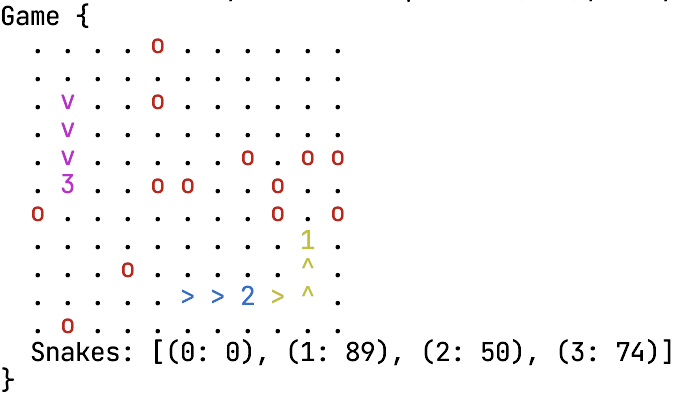
\includegraphics[width=\linewidth]{game_render_eg2.png}\\[12pt]
    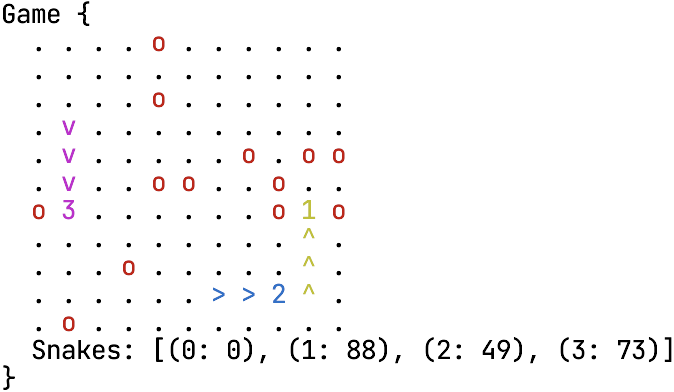
\includegraphics[width=\linewidth]{game_render_eg3.png}
    \caption{ANSI rendering of the game simulation after removing return values
        for dead agents. The lower figure is one step after the upper figure.
    }
    \label{fig:render2}
\end{figure}

We also inspected the behavior of a model trained for 100,000 steps.
This model does not yet seem to be able to avoid colliding with walls.
After training for 1,000,000 steps,
the model is able to avoid walls by circling the grid in a clockwise manner,
opposite to the previous case. Therefore,
it seems that the model needs more training steps to learn proper behaviors,
and an easily reachable local optimum is circling the grid.

\paragraph{VGG-like Model}
The VGG-like model took around 2000 seconds to train for $16^4$ steps using all
CPU cores on the aforementioned server,
about 10 times longer than the MLP model. However, it performed poorly,
even after we added the residual layer, and trained for $51 \times 16^4$ steps.
During manual inspection, the model cannot even consistently avoid walls,
which we consider a rudimentary learning task.
We suspect that the convolutional layers loose the positional information,
which is particularly significant in our case,
because our feature extraction steps center the snake's head in the feature
matrices. Alternatively,
another great possibility is the model requires much more training steps due to
its significantly larger size. Though,
we gave up on further training the VGG-like model because of the known
limitations of CNNs that they require a large amount of data to train.

\paragraph{Impact of Entropy Bonus on Model Performance}
If trained without any entropy bonus,
larger models have a tendency to instruct the snake to spin in a circle
(Figure~\ref{fig:render}).
The deeper MLP model converged to go in a tight circle by keep turning left,
after less than $3\times 16^4$ steps, and all future models remained so.
Similarly,
we observed that the ViT model stays in a tight left-turn circle when the
snake gets into certain positions,
after the model is trained for $72\times 16^4$ steps.
Convergence to spinning happens because of lack of exploration.
At the beginning of training,
the model cannot avoid walls or other snakes consistently,
therefore spinning produces better results than moving around because it avoids
running into walls or snakes, despite making the snake starve to death.
Since there is no entropy bonus,
the model never has a chance to explore better moves,
and eventually converges to spinning.

\begin{figure}
    \centering
    \includegraphics[width=\linewidth]{deep-mlp-spin-render.png}\\[24pt]
    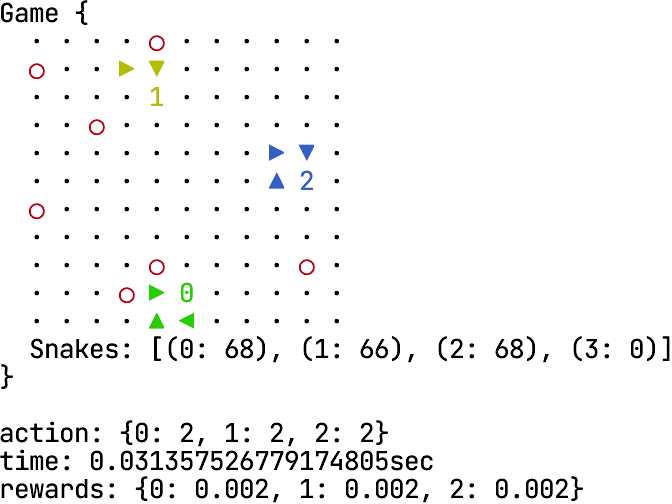
\includegraphics[width=\linewidth]{vit_spin_render.png}
    \caption{Game rendering of the deeper MLP model (upper)
        and the small ViT model (lower) spinning in a circle.
    }
    \label{fig:render}
\end{figure}

We tried to encourage exploration by adding an entropy bonus to the model.
However, after setting the entropy coefficient to 0.1,
our small ViT model could not learn to avoid walls even after training for
$32\times 16^4$ steps. Therefore,
we decided to lower the entropy coefficient to 0.01,
which resulted in our ViT model learning to spin again,
but reach for food when its health is low.
The deeper MLP model learned to spin after sufficient training,
no matter the entropy coefficient.

After we fixed the loading of previous models, added the food reward,
and increased the entropy coefficient to 0.1,
we trained the small ViT model for $865\times 16^4$ steps and the big ViT model
for $429\times 16^4$ steps (counting previous steps trained). However,
the small ViT model still has a less intense tendency to spin,
while neither models can avoid themselves consistently.
Training the small ViT model for $16^4$ steps on an RTX 3090 takes around 580s,
and training the big ViT model for $16^4$ steps takes around 1300s.
We note that the major bottleneck in training is the training efficiency and
getting enough training steps for the model to converge.

\paragraph{Tiny ViT Model}
Based on the results of the small and big ViT models,
we concluded that the models are too large and complex to train effectively,
and we do not have enough resources to train them to convergence,
therefore we focused on training the tiny ViT model instead.

We made large adjustments to the training process of the tiny ViT model to
improve both model performance and training efficiency.
Entropy coefficient is set to a high 0.1 from the beginning,
which is important to prevent the model from converging to spinning.
The learning rate $2\times 10^{-2}$, much larger than $3\times 10^{-4}$,
the training rate previously models used.
We also increased the batch size to 64 from 8192 in an attempt to maximize the
GPU utilization.
Although the real batch size is around 2048 because of the number of steps the
model simulates during each rollout,
increasing the batch size sped up the training of each $16^4$ steps from around
308s to around 214s on an RTX 3090.

The tiny ViT model is mostly able to avoid walls and themselves after only
$134\times 16^4$ steps of training.
It is able to self-play for extended periods of time without spinning or dying
quickly. However,
it is still not able to consistently avoid other snake even after $1000\times
    16^4$ steps of training. Additionally,
the tiny ViT model has a tendency of staying closely together with other agents,
and collide with them, as shown in Figure~\ref{fig:tiny-vit-close-render}

\begin{figure}
    \centering
    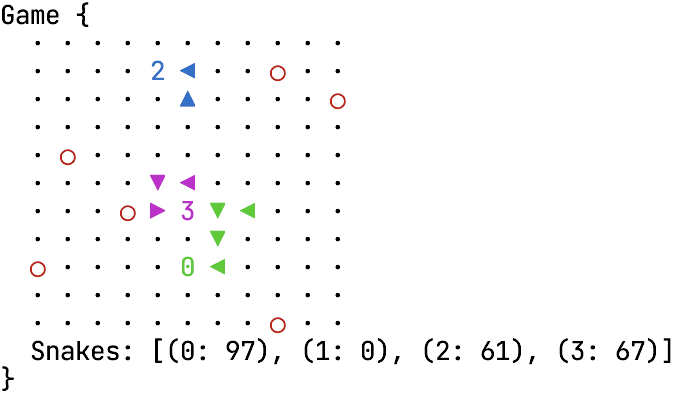
\includegraphics[width=\linewidth]{tiny_vit_close_render.png}
    \caption{Game rendering of the tiny ViT model staying close with other
        agents.
    }
    \label{fig:tiny-vit-close-render}
\end{figure}

\subsubsection{Comparison with max\textsuperscript{n} Tree Search}

For the results,
we anticipated the agent to have comparable performance to tree-search-based
agents,
and planed to benchmark our agent against an open-source tree-search-based agent
implementation consistently ranking top 8 in the standard
leaderboard~\cite{wrenger2024rusty}.
We attempted to test the models against the tree-search-based agent. However,
the tree-search-based agent does not make simple mistakes like running into
other snakes bodies when it has a choice,
therefore the models can never win against the tree search agent in our
observation. We suspect this is why~\cite{chung2020battlesnake}
does not use standard agents as comparison and rather compare the models against
themselves. Therefore,
we do not evaluate the models against the tree-search-based agent.
It would be feasible to evaluate our models against each other, however,
we deem it counterproductive and instead focused our effort in evaluating the
hybrid strategy using the Battlesnake leaderboard~\cite{standard_leaderboard}.

\subsubsection{Hybrid Strategy Real-World Performance}

We first tested our web server against default agents provided on the
Battlesnake website,
then joined the leaderboard and competed with other players for one day.

In our initial testing using $C_o=\frac{1}{2}$,
and without pruning the leaf states,
the algorithm is only able to conduct a search of depth 1.
We analyze and find that majority of time is spent on neural network inference,
which,
since our model inference is around 1.2ms for all four players' observations,
limits our available state evaluation chances to around less than 90.
After we massively reduced the search span by setting $C_o=\frac{3}{4}$ and
adding the leaf state pruning,
the algorithm is able to consistently search to depth 2 or 3,
and occasionally to depth 8 when there are fewer valid states.
We note that the Python Global Interpreter Lock and PyO3's implementation blocks
our implementation to utilize more than one CPU cores,
and elevating this limitation should increase its computational capacity by
around $2\times$.

Our real-world test in the Battlesnake leaderboard is successful,
but with significance less than desired. During the one-day test,
our agent won all 99 games except for one game where the web server web
temporarily shut down,
and one game where it failed to respond within 500ms potential due to unexpected
network lag. However, all of the games are within 11 steps,
with trivial opponents that either only go up,
or conduct suicide\footnote{We found an agent named ``The Worst Possible Snake
    '' that tries to collide with walls or its own body as quickly as
    possible.}.
Therefore, the results demonstrate that our methods are reliable and practical,
but only for low-level game play.

\todo{analyze the experimental data accordingly}

\section{Conclusion and Future Work}

We developed purely deep-reinforcement-learning-based Battlesnake
agent capable of operating in resource-constrained environments like low-tier
cloud VMs.
Trained with custom simulation environment and modified Proximal Policy Optimization implementation,
our agents learned to avoid walls and themselves.
We combine the agents with tree search into a hybrid strategy,
and succeeded in competing on the standard Battlesnake leaderboard.
Despite the success on a basic level,
the model and the training process have much room for improvement. Especially,
training complex neural networks to convergence is a major bottleneck,
and our agents are not yet able to consistently avoid other snakes.
We believe our basic methods of training reinforcement learning agents with only
knowledge provided by the simulation environment are sound,
and further training and tuning will improve the agents' performance to meet
high-level game play.

\printbibliography

\end{document}
